\documentclass[12pt]{extarticle}
\usepackage{tempora}
\usepackage[T1, T2A]{fontenc}
\usepackage[utf8]{inputenc}
\usepackage[english, ukrainian]{babel}
\usepackage{geometry}
\usepackage{graphicx}
\usepackage{multirow}
\usepackage{multicol}
\usepackage{float}
\usepackage{indentfirst}
\graphicspath{{/home/artem/Pictures}}
\geometry
{
    a4paper,
    left=30mm,
    top=15mm,
    right=20mm,
    bottom=15mm,
}

\begin{document}
\begin{titlepage}
    \begin{center}
        \textbf{\normalsize{\MakeUppercase{
            Міністерство Освіти і науки України
            Національний університет "Львівська політехніка"
        }}}

        \begin{flushright}
        \textbf{ІКНІ}\\
        Кафедра \textbf{ПЗ}
        \end{flushright}
        \vspace{15mm}

        \includegraphics[width=0.4\textwidth]{lpnu_logo.png}

        \vspace*{\fill}

        \textbf{\normalsize{\MakeUppercase{Звіт}}}
            
        До лабораторної роботи №11

        \textbf{на тему:} “Дослідження та робота з таблицею маршрутизації у Windows XP.”

        \textbf{з дисципліни:} “Організація комп'ютерних мереж”
            
        \vspace*{\fill}

        \begin{flushright}

            \textbf{Лектор:}\\
            доцент кафедри ПЗ\\
            Крук О.Г.\\
            \vspace{12pt}

            \textbf{Виконав:}\\
            студент групи ПЗ-24\\
            Губик А. С.\\
            \vspace{12pt}

            \textbf{Прийняв:}\\
            доцент кафедри ПЗ\\
            Задорожний І. М.\\
        \vspace{12pt}
        \end{flushright}

        Львів -- 2023
            
            
    \end{center}
\end{titlepage}

\textbf{Тема роботи:} Дослідження та робота з таблицею маршрутизації у Windows XP.
\vspace{12pt}

\textbf{Мета роботи:} Ознайомитися з принципами маршрутизації та навчитися користуватися утилітою
route для зміни таблиці маршрутизації вручну.

\subsection*{Теоретичні відомості}
Як відзначалося у попередній лабораторній роботі, на протоколі IP лежить
відповідальність за маршрутизацію. Нагадаємо, що маршрутизація – це вибір маршруту
передачі IP-пакетів в мережі (процес вибору маршруту ще називають IP-роутингом). Цей
вибір здійснюється на основі розглянутих нижче принципів. У виборі маршруту беруть
участь не лише маршрутизатори, але й кінцеві вузли (комп’ютери).
Маршрутизація можу бути безпосередньою (direct) та опосередкованою (indirect).
Безпосередня маршрутизація здійснюється без участі маршрутизатора у випадку, якщо вузол
відправник IP-пакета та вузол-одержувач належать одній підмережі (як ми знаємо, фізичну
адресу вузла-одержувача отримуємо за допомогою протоколу ARP). Опосередкована
маршрутизація – більш типовий випадок, вона виконується тоді, коли вузол-відправник і
вузол-одержувач належать різним підмережам.
При опосередкованій маршрутизації рішення про те, кому передати пакет, робиться
на основі таблиць маршрутизації (routing tables). При цьому у стеку TCP/IP застосовується
підхід, при якому кожен маршрутизатор (або кінцевий вузол) вибирає лише один крок
передачі пакета, тобто, лише адресу того іншого маршрутизатора, якому буде скерований
пакет (в англомовній літературі цей підхід носить назву next-hop routing). Тоді цей інший
маршрутизатор вибиратиме наступний крок маршрутизації і т.д. При однокроковому підході
до маршрутизації пакетів немає обмеження на кількість маршрутизаторів, що лежать на
шляху пакета.
Існує і інший підхід до маршрутизації – маршрутизація від джерела (Source Routing),
при якому вся послідовність маршрутизаторів на шляху пакета задається наперед або
кінцевим вузлом-відправником пакета, або першим маршрутизатором. Цей підхід
застосовується в IP-мережах лише для відлагодження. Маршрут прописується у вже
відомому нам полі IP-опції IP-пакета.
Таблиця маршрутизації має фіксований формат. Типовий приклад таблиці
маршрутизації представлений таблицею 1. Звісно, таблиця такого типу є в кожного
маршрутизатора і кінцевого вузла (але дані в кожній такій таблиці свої). Однак, створюються
такі таблиці по-різному для маршрутизаторів і кінцевих вузлів. Для кінцевого вузла
характерне заповнення таблиці маршрутизації вручну (адміністраторами) і збереження їх у
вигляді файлів на дисках. Натомість маршрутизатори типово формують таблиці
маршрутизації автоматично, на основі обміну службової інформації. Існує три класи
алгоритмів побудови однокрокової маршрутизації: алгоритми фіксованої маршрутизації;
алгоритми простої маршрутизації; алгоритми адаптивної маршрутизації.
Таблиці маршрутизації в маршрутизаторів є значно більші, ніж у кінцевих вузлів.

\break
\subsection*{Хід роботи}
\paragraph{2.}.

\vspace{12pt}

\begin{figure}[H]
    \centering
    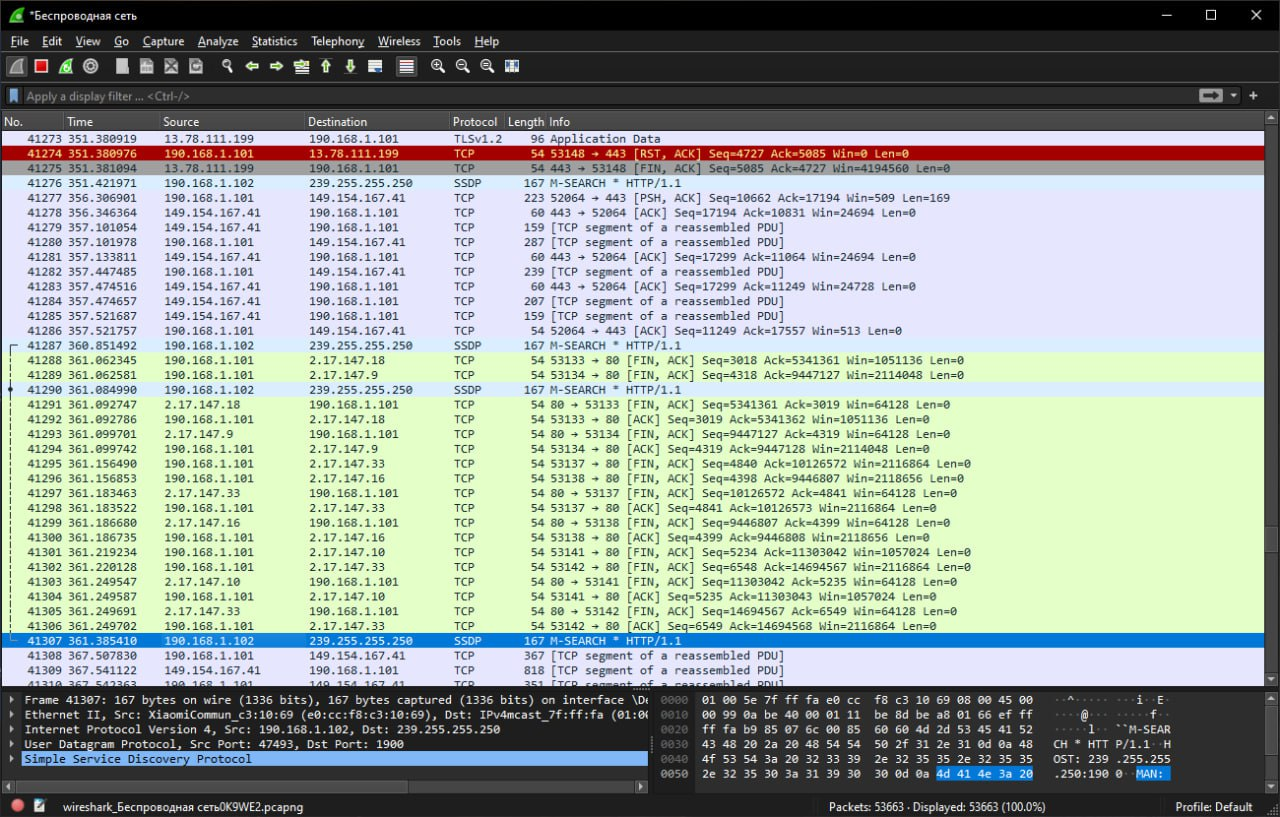
\includegraphics[width=0.90\textwidth]{ips}
    \caption{Перелік пакетів}
\end{figure}


\paragraph{3.}.
\begin{figure}[H]
    \centering
    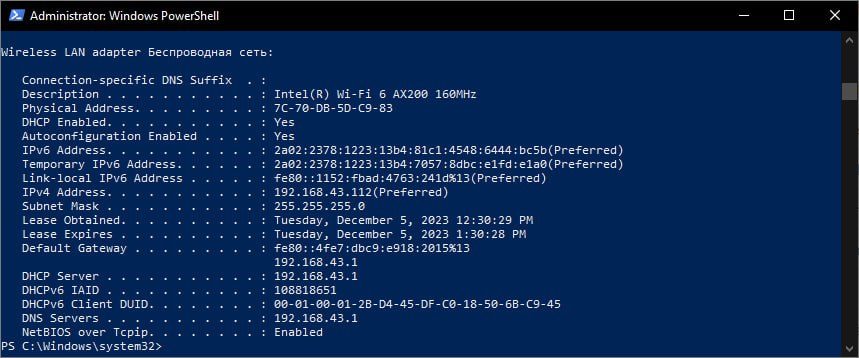
\includegraphics[width=0.90\textwidth]{ipconfig}
    \caption{ipconfig}
\end{figure}

Як бачимо наш ІР адрес 192.168.43.112, маска 255.255.255.0, тобто
в мережу може входити 255 адрес від 192.168.43.0 до 192.168.43.255.

\break
\paragraph{4.}.

\begin{figure}[H]
    \centering
    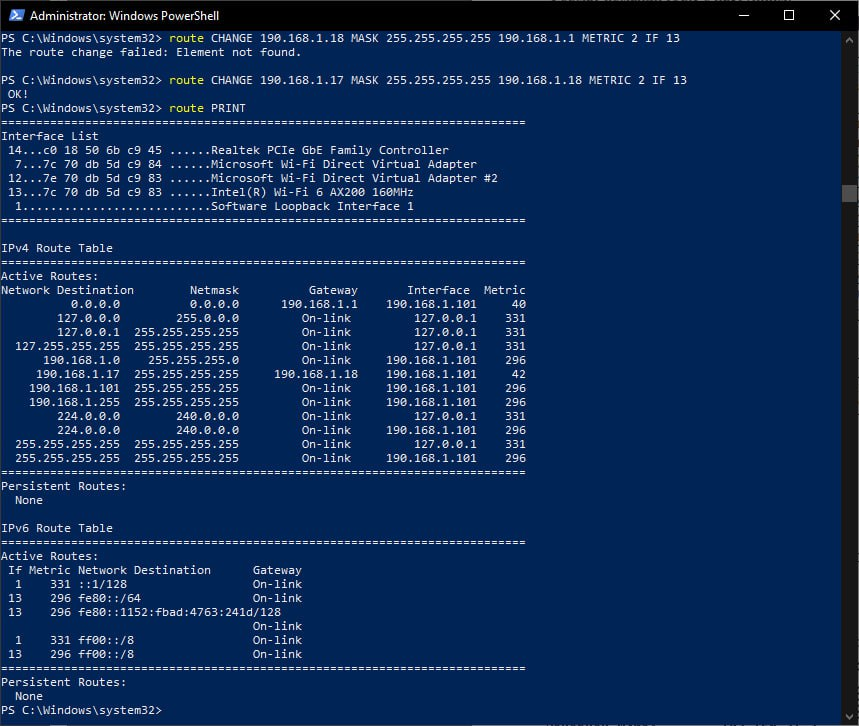
\includegraphics[width=0.90\textwidth]{route_print}
    \caption{}
\end{figure}

\begin{figure}[H]
    \centering
    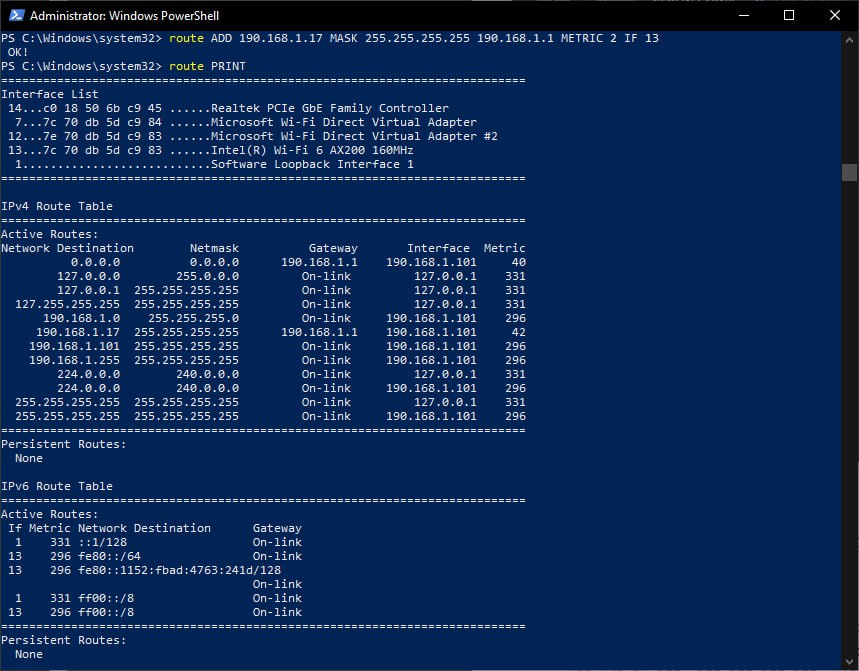
\includegraphics[width=0.90\textwidth]{route_add}
    \caption{}
\end{figure}

\begin{figure}[H]
    \centering
    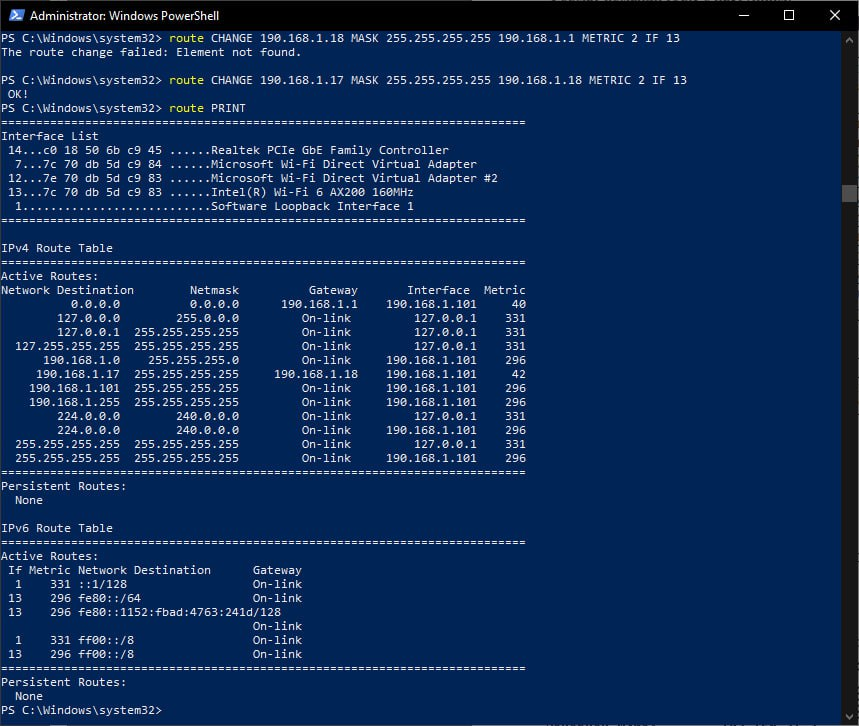
\includegraphics[width=0.90\textwidth]{route_change}
    \caption{}
\end{figure}

\begin{figure}[H]
    \centering
    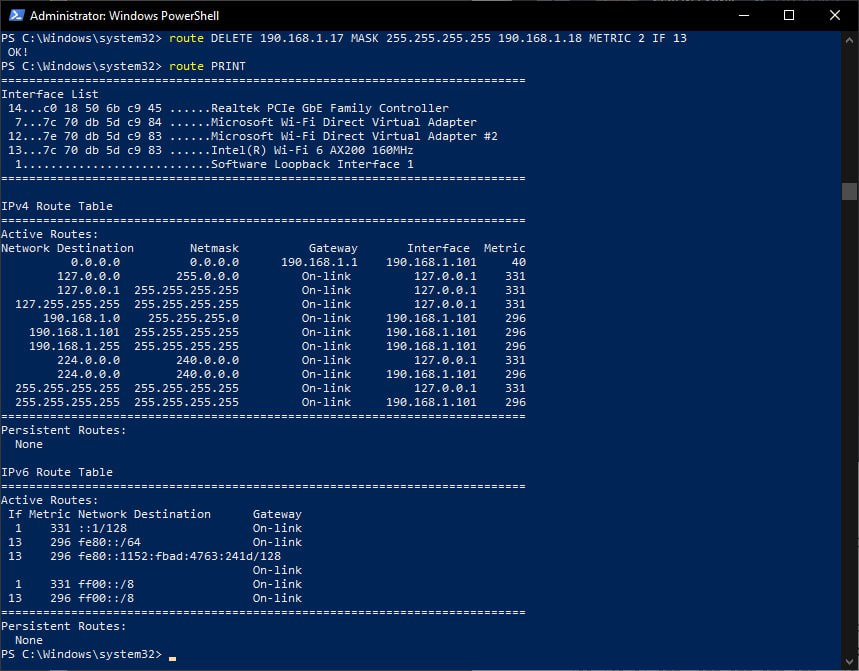
\includegraphics[width=0.90\textwidth]{route_delete}
    \caption{}
\end{figure}


\paragraph{5.}.

\begin{figure}[H]
    \centering
    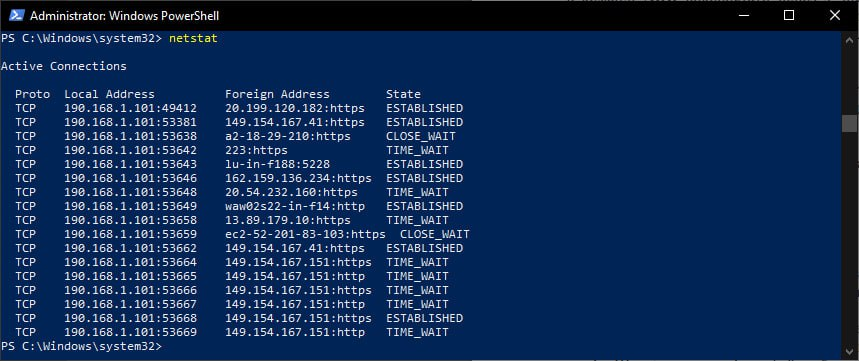
\includegraphics[width=0.90\textwidth]{netstat}
    \caption{}
\end{figure}

\paragraph{6.}.
Поле інтерфейсу означає мережевий інтерфейс. Він ідентифікується мак адресом,
але так як це інтернет, то мак адрес не має для нас ніякої цінності, в інтернеті 
працюють ІР-адреси.

\paragraph{7.}.
IGMP, (англ. Internet Group Management Protocol — протокол керування групами Інтернету) — протокол керування груповою (multicast) передачею даних в мережах, базованих на протоколі IP. IGMP використовується маршрутизаторами і IP-точками для об'єднання мережевих пристроїв в групи.

Цей протокол є частиною специфікації групової передачі пакетів в IP-мережах. IGMP розташований вище мережевого рівня, хоча, насправді, функціонує не як транспортний протокол. Він в багато чому аналогічний ICMP для односторонньої передачі. IGMP може використовуватись для підтримки потокового відео і онлайн-ігор, для таких типів програм він дозволяє використовувати ресурси мережі ефективніше. 

\vspace{12pt}

\subsection*{Висновок} 
Я навчився як користуватись командою route i netstat, що таке таблиця 
маршрутизації і як її можна змінювати.
\end{document}